% Copyright (c) 2022 by Lars Spreng
% This work is licensed under the Creative Commons Attribution 4.0 International License. 
% To view a copy of this license, visit http://creativecommons.org/licenses/by/4.0/ or send a letter to Creative Commons, PO Box 1866, Mountain View, CA 94042, USA.

%~~~~~~~~~~~~~~~~~~~~~~~~~~~~~~~~~~~~~~~~~~~~~~~~~~~~~~~~~~~~~~~~~~~~~~~~~~~~~~
% You can add your packages and commands to the loadslides.tex file. 
% The files in the folder "styles" can be modified to change the layout and design of your slides.
% I have included examples on how to use the template below. 
% Some of it these examples are taken from the Metropolis template.
%~~~~~~~~~~~~~~~~~~~~~~~~~~~~~~~~~~~~~~~~~~~~~~~~~~~~~~~~~~~~~~~~~~~~~~~~~~~~~~


\documentclass[
11pt,notheorems,compress,hyperref={pdfauthor=Maghfira Ramadhani}
]{beamer}


% Copyright (c) 2022 by Lars Spreng
% This work is licensed under the Creative Commons Attribution 4.0 International License. 
% To view a copy of this license, visit http://creativecommons.org/licenses/by/4.0/ or send a letter to Creative Commons, PO Box 1866, Mountain View, CA 94042, USA.

%~~~~~~~~~~~~~~~~~~~~~~~~~~~~~~~~~~~~~~~~~~~~~~~~~~~~~~~~~~~~~~~~~~~~~~~~~~~~~~
% Add your packages and commands to this file
%~~~~~~~~~~~~~~~~~~~~~~~~~~~~~~~~~~~~~~~~~~~~~~~~~~~~~~~~~~~~~~~~~~~~~~~~~~~~~~

%~~~~~~~~~~~~~~~~~~~~~~~~~~~~~~~~~~~~~~~~~~~~~~~~~~~~~~~~~~~~~~~~~~~~~~~~~~~~~~
\RequirePackage{palatino}
\RequirePackage[utf8]{inputenc}
\RequirePackage[T1]{fontenc}

\usefonttheme{serif}

\usepackage{styles/elegantmacros}
\usefolder{styles}
\usetheme[style=blue]{elegant}

\newcommand{\makepart}[1]{ % For convenience
\part{#1} \frame{\partpage}
}

%~~~~~~~~~~~~~~~~~~~~~~~~~~~~~~~~~~~~~~~~~~~~~~~~~~~~~~~~~~~~~~~~~~~~~~~~~~~~~~

%~~~~~~~~~~~~~~~~~~~~~~~~~~~~~~~~~~~~~~~~~~~~~~~~~~~~~~~~~~~~~~~~~~~~~~~~~~~~~~
% Figures
\RequirePackage{booktabs}
\RequirePackage{colortbl}
\RequirePackage{ragged2e}
\RequirePackage{schemabloc}
%\RequirePackage{natbib}
\RequirePackage{caption}
\RequirePackage{subcaption}
\RequirePackage{tabularx}
\RequirePackage{array}
\RequirePackage{multirow}
\usepackage[
  style=authoryear, 
]{biblatex}
\addbibresource{references.bib}
\newcolumntype{Y}{>{\centering\arraybackslash}X}

%~~~~~~~~~~~~~~~~~~~~~~~~~~~~~~~~~~~~~~~~~~~~~~~~~~~~~~~~~~~~~~~~~~~~~~~~~~~~~~

%~~~~~~~~~~~~~~~~~~~~~~~~~~~~~~~~~~~~~~~~~~~~~~~~~~~~~~~~~~~~~~~~~~~~~~~~~~~~~~
% Figures
\RequirePackage{wrapfig}
\RequirePackage{pgfplots}
\RequirePackage{graphicx}
\RequirePackage{adjustbox}
\RequirePackage{environ}
\pgfplotsset{compat=1.18}

\makeatletter
\newsavebox{\measure@tikzpicture}
\NewEnviron{scaletikzpicturetowidth}[1]{%
  \def\tikz@width{#1}%
  \def\tikzscale{1}\begin{lrbox}{\measure@tikzpicture}%
  \BODY
  \end{lrbox}%
  \pgfmathparse{#1/\wd\measure@tikzpicture}%
  \edef\tikzscale{\pgfmathresult}%
  \BODY
}
\makeatother
%~~~~~~~~~~~~~~~~~~~~~~~~~~~~~~~~~~~~~~~~~~~~~~~~~~~~~~~~~~~~~~~~~~~~~~~~~~~~~~

%~~~~~~~~~~~~~~~~~~~~~~~~~~~~~~~~~~~~~~~~~~~~~~~~~~~~~~~~~~~~~~~~~~~~~~~~~~~~~~
% Maths 
\RequirePackage{textcomp}
\RequirePackage{amsmath} 
\RequirePackage{amsthm}
\RequirePackage{mathtools}
%\RequirePackage{bbm}
%\RequirePackage{algorithm}
%\RequirePackage[osf,sc]{mathpazo}
%\RequirePackage{pifont}
%\newcommand{\xmark}{\ding{55}}%
%\numberwithin{equation}{section}
\DeclareMathOperator*{\argmax}{arg\,max}
\DeclareMathOperator*{\argmin}{arg\,min}

\setbeamertemplate{theorems}[numbered] % to number

\theoremstyle{definition}
\newtheorem{fact}{Fact}[section]
\newtheorem{examp}{Example}[section]

\theoremstyle{plain}
\newtheorem{definition}{Definition}[section]
\newtheorem{proposition}{Proposition}
\newtheorem{theorem}{Theorem}
\newtheorem{assumption}{Assumption}

\providecommand{\H}{\mathscr{H}}      
\providecommand{\E}{\mathbb{E}}
\makeatletter
\def\munderbar#1{\underline{\sbox\tw@{$#1$}\dp\tw@\z@\box\tw@}}
\makeatother

%~~~~~~~~~~~~~~~~~~~~~~~~~~~~~~~~~~~~~~~~~~~~~~~~~~~~~~~~~~~~~~~~~~~~~~~~~~~~~~
 % Loads packages and some defined commands

\title[
% Text entered here will appear in the bottom middle
]{Improving Rural Accessibility in Indonesia: Fuel Subsidy versus Infrastructure Development}

\author[
% Text entered here will appear in the bottom left corner
]{
    Maghfira Ramadhani 
}

\institute{
    School of Economics, \\
    Georgia Institute of Technology}
\date{\today}

\begin{document}

% Generate title page
{
\setbeamertemplate{footline}{}
\begin{frame}
  \titlepage
\end{frame}
}
\addtocounter{framenumber}{-1}

% You can declare different parts as a parentof sections
\section{Introduction}
{
\setbeamertemplate{footline}{}
\begin{frame}{Outline}
    \tableofcontents%[part=1]
\end{frame}
}
%\makepart{Proposal}

\begin{frame}
    Unless the user enters their own custom frame titles and subtitles, Elegant Slides automatically inserts the section title and, if specified, the subsection title as frame titles and frame subtitles.
\end{frame}

\subsection{Research Question}
\begin{frame}
\begin{itemize}
    \item infrastructure \up \so cost \up \citet{hartojo_2022}
    \item This paper builds on literature on rural development and fossil fuel subsidy in Indonesia. Related literature has indicated that both subsidizing fuel and inter-government transfer has contributed to improving accessibility in rural areas. 
    \item This research measures the magnitude of these mechanisms and tests whether they are complementary or supplementary. From a political economy perspective, infrastructure development is managed by the government directly, while the fuel subsidy is managed through the National Oil Company (NOC) as a delivery agent \citet{ichsan_2022}. This research exercises the cost-benefit of the options to substantially inform decision-makers.
\end{itemize}
\end{frame}

\section{Institutional Context and Conceptual Framework}
\subsection{Transportation structure in rural area}
\begin{frame}
\begin{itemize}
    \item Developing countries have been focusing on decentralization and local government reform with the belief that they are \alert{\textbf{more efficient}} in bringing local development (\citet{vazquez_2017}) 
    \item 
    \item 
\end{itemize}
\end{frame}

\subsection{Fossil fuel subsidy regime}
\begin{frame}
    This frame has a custom title and a custom subtitle. \footnote{This is a footnote. See also \citet{hartojo_2022}. }
\end{frame}

\subsection{Decentralization of development}
\begin{frame}
    This frame has a custom title and a custom subtitle. \footnote{This is a footnote. See also \citep{hartojo_2022}. }
\end{frame}


\begin{frame}
    \begin{figure}[t]
    \subcaptionbox{Village status in 2014\label{f:panel1}}{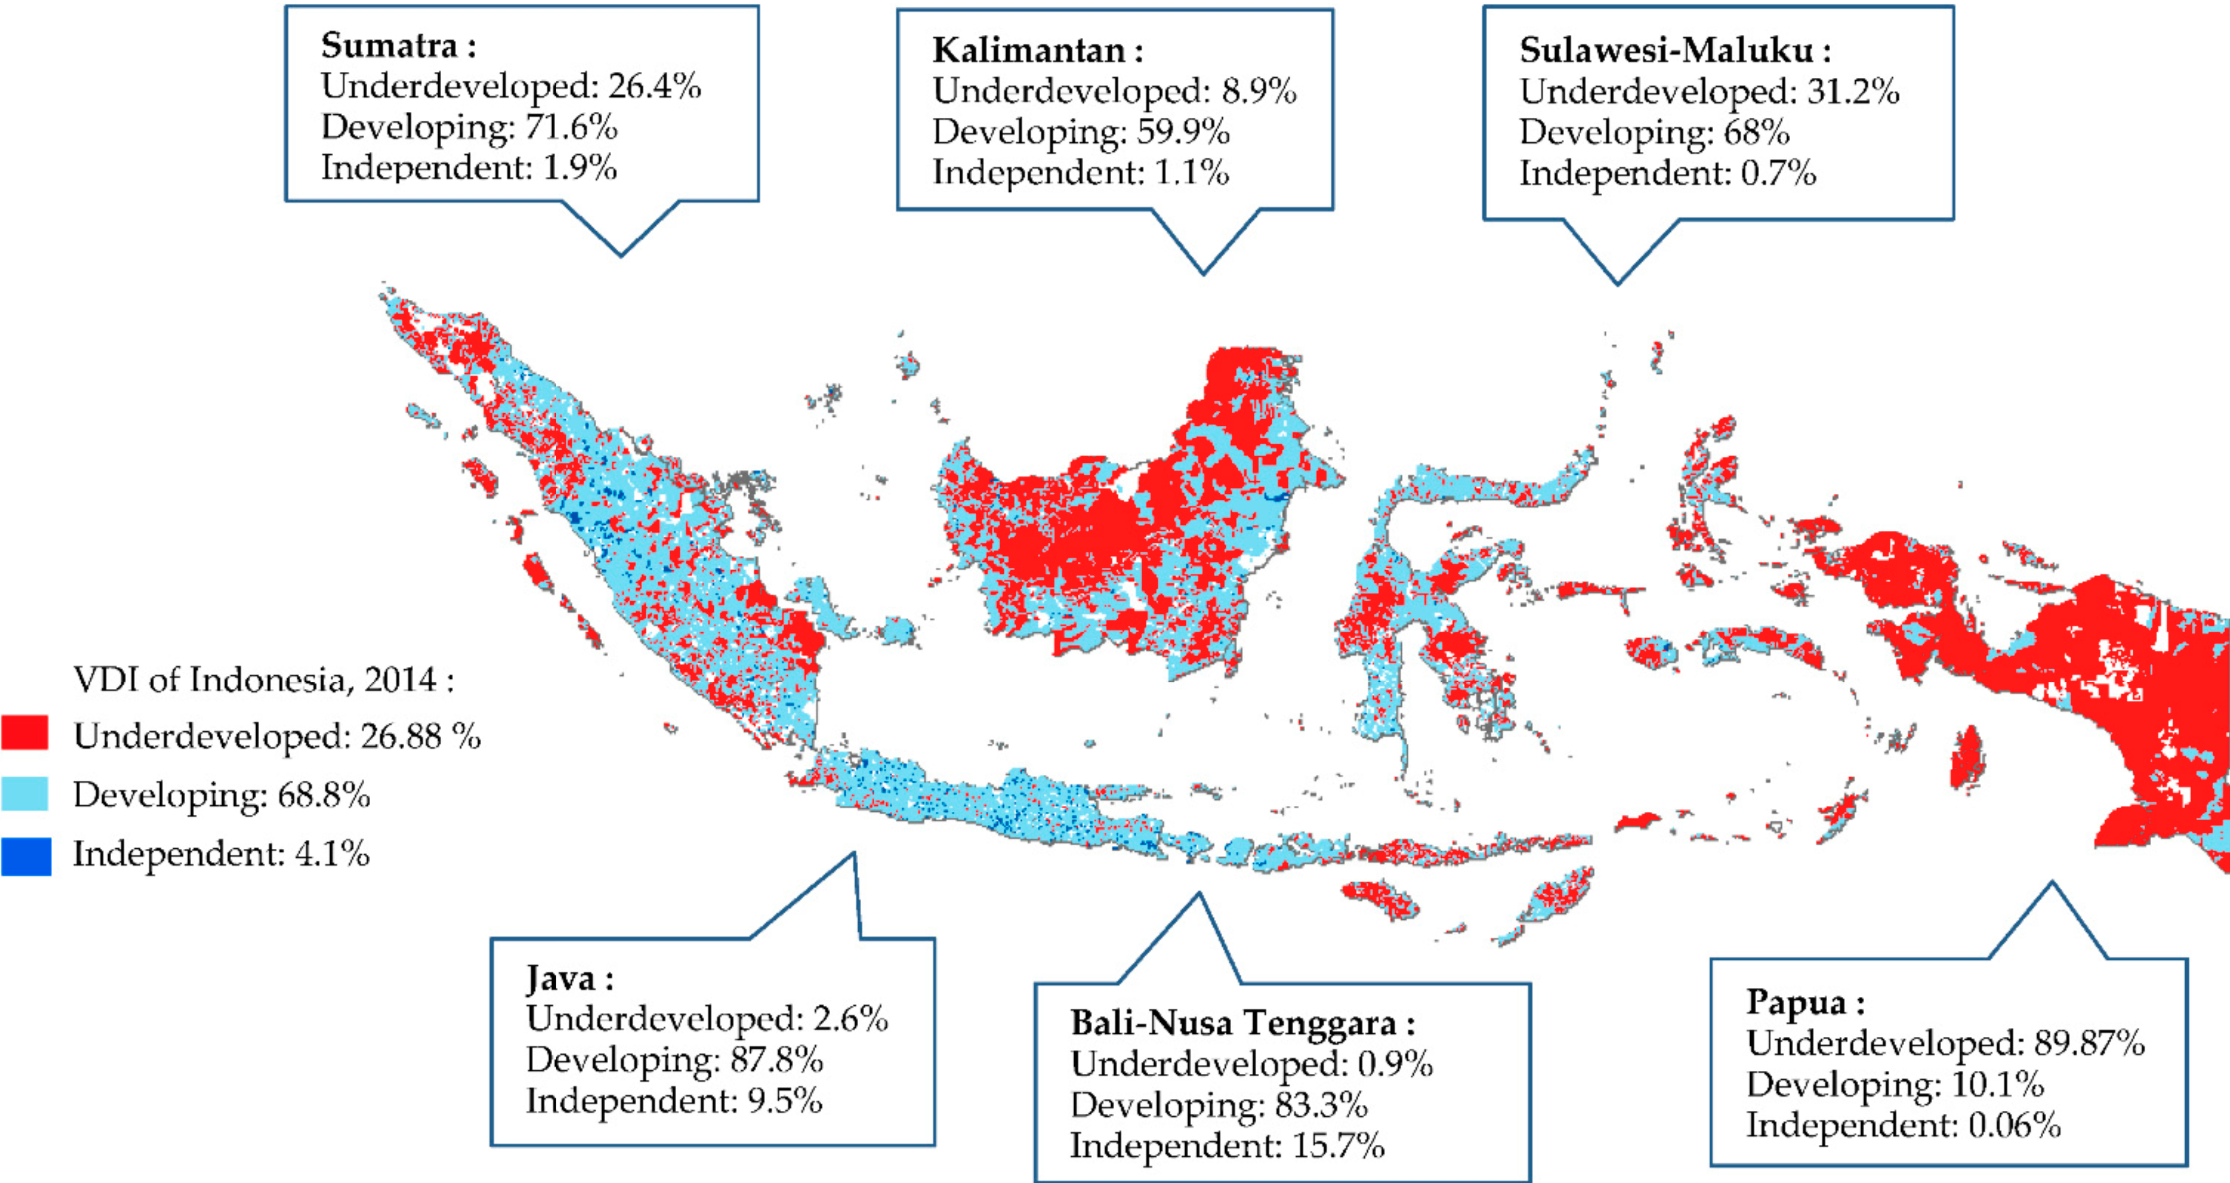
\includegraphics[scale=0.2]{Final_Project/image/vdi2014.png}}\hfill
    \subcaptionbox{Village status in 2018\label{f:panel2}}{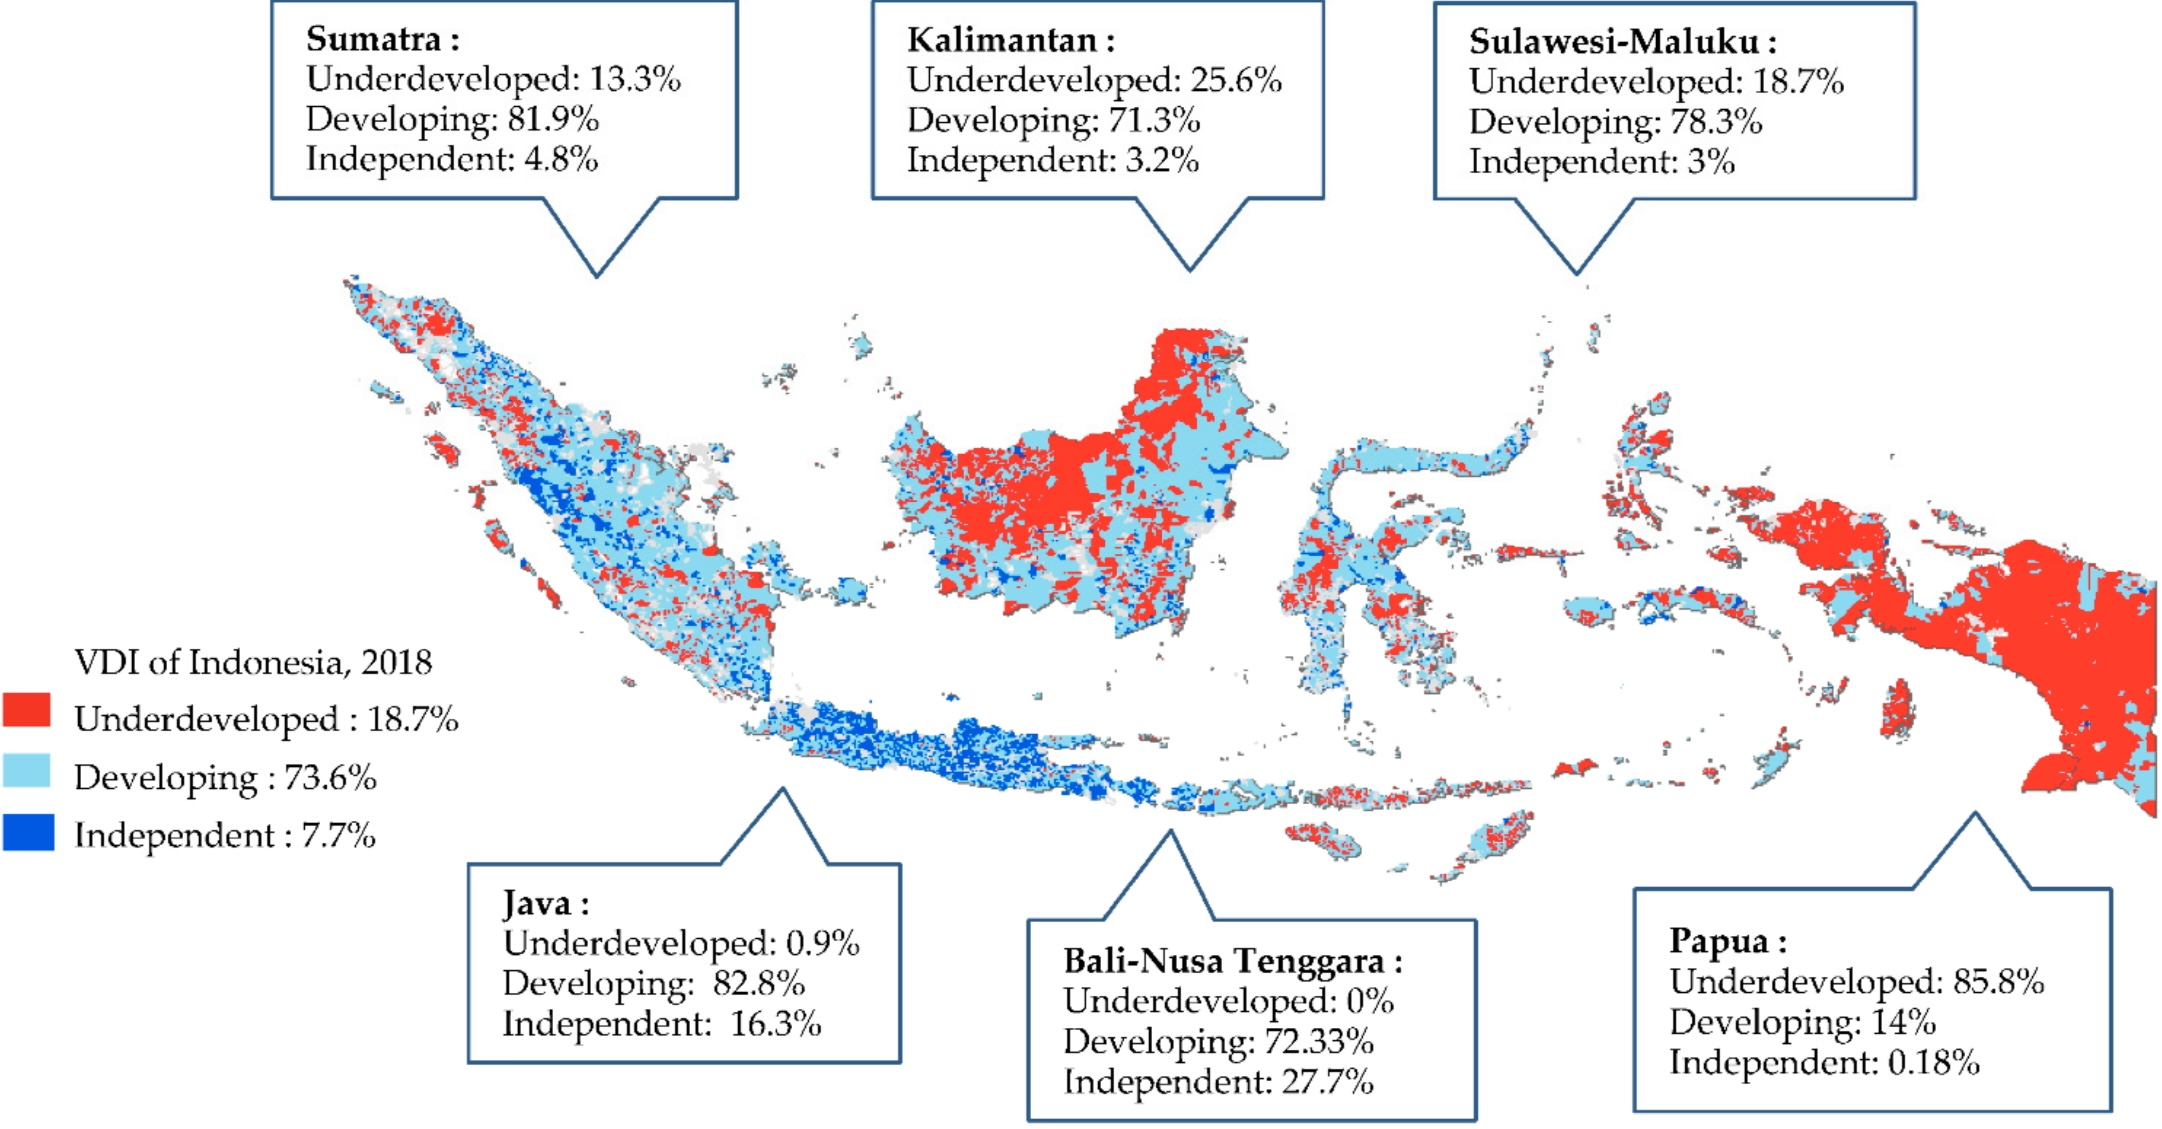
\includegraphics[scale=0.205]{Final_Project/image/vdi2018.jpg}}
    \caption{Indonesia's VDI's status}
    \note{Source: Statistics Indonesia \citet{hartojo_2022}}
    \label{f:graph1}
    \end{figure}
\end{frame}

\section{Data}
\subsection{Data Description}
\begin{frame}
    \begin{itemize}
        \item I obtained the \al{Village Potential Statistics} data for the year 2014 and 2018 from Indonesia's Central Bureau of Statistics complemented with village fund transfer data form Ministry of Village Development.
        \item I measure rural accessibility using the \al{unit transportation cost} (in Rp/km) of each individual village. 
        \footnote{I define unit transportation cost, $y_{it}$, as the \al{transportation cost} from the village office to the sub-district office (in thousands Rp), $c_{it}$, divided by the \al{distance} from the village office to the sub-district office (in km), $d_{it}$.
        \begin{equation}
        y_{it}=\frac{d_{it}}{c_{it}}    
        \end{equation}}
        \item I define the treatment group as the
    \end{itemize}
\end{frame}

\subsection{Summary Statistics}
\begin{frame}
    \begin{table}[h]
    \caption{Summary statistics of main variables. }
    \scalebox{0.75}{\begin{tabular}{l*{2}{ccccc}}
\toprule
                &     2014&         &         &         &         &     2018&         &         &         &         \\
                &     Mean&     S.D.&      Min&      Max&     Obs.&     Mean&     S.D.&      Min&      Max&     Obs.\\
\midrule
\emph{Transportation Cost}&         &         &         &         &         &         &         &         &         &         \\
\hspace{0.25cm} Unit transportation cost in 000s Rp./km&    22.35&   304.78&     0.00& 25000.00&    65917&     3.52&    29.19&     0.00&  5000.00&    65934\\
\hspace{0.25cm} Transportation cost in 000s Rp.&   106.42&  1205.17&     0.00& 55000.00&    65917&    35.41&   325.19&     0.00& 50000.00&    65934\\
\vspace{0.05em} \\ \emph{Natural Disaster}&         &         &         &         &         &         &         &         &         &         \\
\hspace{0.25cm} Landfall occurence average per year&     0.10&     0.50&     0.00&     9.00&    65917&     0.14&     0.61&     0.00&     9.00&    65934\\
\hspace{0.25cm} Earthquake occurence average per year&     0.06&     0.41&     0.00&     9.00&    65917&     0.21&     0.91&     0.00&     9.00&    65934\\
\vspace{0.05em} \\ \emph{Infrastructure}&         &         &         &         &         &         &         &         &         &         \\
\hspace{0.25cm} Number of PLN electricity user household&   679.68&   871.06&     0.00& 19714.00&    65917&   769.27&   988.12&     0.00& 23755.00&    65934\\
\hspace{0.25cm} Number of Junior High School&     0.55&     0.83&     0.00&    22.00&    65917&     0.60&     0.88&     0.00&    12.00&    65934\\
\hspace{0.25cm} Number of Senior High School or Vocational High School&     0.28&     0.71&     0.00&    40.00&    65917&     0.34&     0.77&     0.00&    13.00&    65934\\
\vspace{0.05em} \\ \emph{Inter-government Transfer}&         &         &         &         &         &         &         &         &         &         \\
\hspace{0.25cm} Revenue from village fund transfer&   115.53&   203.86&     0.00&  7792.00&    65917&   117.93&   127.47&     0.00& 13662.00&    63682\\
\bottomrule
\end{tabular}
}
    \label{t1}\end{table}
\end{frame}

\section{Empirical Strategy}
\subsection{Identification}
\begin{frame}

   \centering
	\begin{minipage}[b]{0.5\textwidth}

	  \begin{block}{Default}
        Block content.
      \end{block}

      \begin{alertblock}{Alert}
        Block content.
      \end{alertblock}

      \begin{exampleblock}{Example}
        Block content.
      \end{exampleblock}      
      
	\end{minipage}	
\end{frame}

\subsection{Model Specification}
\begin{frame}

   \centering
	\begin{minipage}[b]{0.5\textwidth}

	  \begin{block}{Default}
        Block content.
      \end{block}

      \begin{alertblock}{Alert}
        Block content.
      \end{alertblock}

      \begin{exampleblock}{Example}
        Block content.
      \end{exampleblock}      
      
	\end{minipage}	
\end{frame}

\section{Results}
\subsection{Main Results}
\begin{frame}
    \begin{columns}[T,onlytextwidth]
    \column{0.33\textwidth}
      \textbf{Items}
      \begin{itemize}
        \item Cats 
        \begin{itemize}
            \item British Shorthair
        \end{itemize}
        \item Dogs \item Birds
      \end{itemize}

    \column{0.33\textwidth}
      \textbf{Enumerations}
      \begin{enumerate}
        \item First 
        \begin{enumerate}
            \item First subpoint
        \end{enumerate}
        \item Second \item Last
      \end{enumerate}

    \column{0.33\textwidth}
      \textbf{Descriptions}
      \begin{description}
        \item[Apples] Yes \item[Oranges] No \item[Grappes] No
      \end{description}
\end{columns}
\end{frame}

\subsection{Robustness}
\begin{frame}
    \begin{columns}[T,onlytextwidth]
    \column{0.33\textwidth}
      \textbf{Items}
      \begin{itemize}
        \item Cats 
        \begin{itemize}
            \item British Shorthair
        \end{itemize}
        \item Dogs \item Birds
      \end{itemize}

    \column{0.33\textwidth}
      \textbf{Enumerations}
      \begin{enumerate}
        \item First 
        \begin{enumerate}
            \item First subpoint
        \end{enumerate}
        \item Second \item Last
      \end{enumerate}

    \column{0.33\textwidth}
      \textbf{Descriptions}
      \begin{description}
        \item[Apples] Yes \item[Oranges] No \item[Grappes] No
      \end{description}
\end{columns}
\end{frame}


\section{Concluding Remarks}
\begin{frame}
    \begin{table}
        \caption{Largest cities in the world (source: Wikipedia)}
        \begin{tabular}{@{} lr @{}}
          \toprule
          City & Population\\
          \midrule
          Mexico City & 20,116,842\\
          Shanghai & 19,210,000\\
          Peking & 15,796,450\\
          Istanbul & 14,160,467\\
          \bottomrule
        \end{tabular}
        \hspace*{1cm}
            \setlength\extrarowheight{3pt}
        \begin{tabular}{|lr|}
          \hline
          \rowcolor{primary}\color{white}City & \color{white}Population\\
          \hline
          Mexico City & 20,116,842\\
          Shanghai & 19,210,000\\
          Peking & 15,796,450\\
          Istanbul & 14,160,467\\
          \hline
        \end{tabular}
    \end{table}
\end{frame}

\section{}
\begin{frame}[allowframebreaks]{References}
    \bibliographystyle{Final_Project/paper/bibliography.bst}
    \bibliography{references.bib}
\end{frame}
\end{document}